\section{Kontrolenhed}
Til Kontrolenheden er der opsat følgende krav:
\begin{enumerate}
	\item Skal kunne kommunikere over Wifi
	\item Skal fungere som streamserver med tilkoblet kamera
	\item Skal kunne kommunikere over I2C
\end{enumerate}

Der er valgt en Raspberry Pi 3 Model B med operativsystemet Raspbian Jessie 4.4.
Denne enhed er valgt, fordi den er let tilgængelig, den har fyldestgørende dokumentation og den er open source. \\
Den opfylder de to første krav fuldt ud, dog er det tredje krav begrænset til, at den udelukkende kan fungere som I2C master. 
Dette gør, at der hele tiden skal polles på porten, for at se om PSoC'en har noget data, som skal videresendes over Wifi. 
Det kunne have været mere intuitivt at bygge det op således, at Pi'en kunne fungere som slave, når den ikke skal sende beskeder. 
På denne måde ville den kun videresende data, når den modtog noget, i stedet for at skulle polle på I2C-porten.

\subsection{Kontrolenhedens Wifi}
PC'en skal kunne kommunikere med Kontrolenheden via TCP-/UDP-protokollerne over Wifi. 
I det færdige produkt er det tiltænkt, at robotten kan befinde sig i dvaletilstand, indtil PC'en opretter forbindelse. 
For at muliggøre dette, er det valgt, at Kontrolenheden skal fungere som et Wifi-hotspot, som PC'en opretter forbindelse til.

Hotspottet bliver sat op ved brug af disse programmer:
\begin{itemize}
	\item \textit{dnsmasq} som er et DNS og DHCP serverprogram.
	\item \textit{hostapd} som kan holde styr på tilladelserne i et Wifi-netværk.
\end{itemize}

Til opsætningen benyttes programmet \textit{RaspAp-Webgui} \cite{raspap}, der benytter ovenstående programmer med en webbaseret brugergrænseflade til at sætte  Pi'en op til at fungere som en router.

\subsubsection{Enhedstest af Kontrolenhedens Wifi}
For at teste router-funktionen, opsættes Pi'en til at oprette et trådløst netværk med SSID og password. 
Med en PC oprettes forbindelse til hotspottet og det verificeres, at forbindelsen bliver oprettet og PC’en modtager en IP-adresse.
\begin{figure} [H]
	\centering
	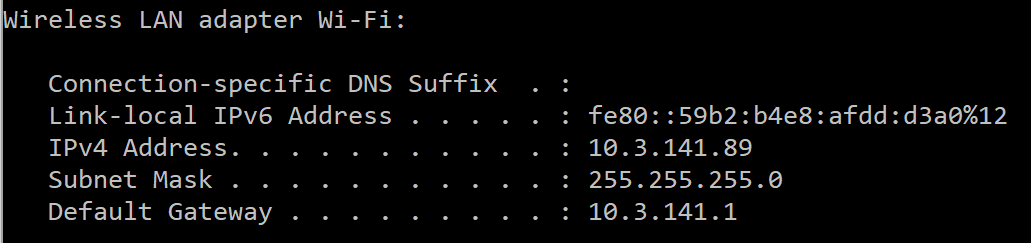
\includegraphics[width=0.7 \textwidth]{test_wifi.png}
	\captionof{figure}{Skærmklip fra PC'ens ipconfig i kommandoprompten ved test af Wifi}
	\label{fig:wifi_test}
\end{figure}
\newpage
På figur \ref{fig:wifi_test} ses et skærmudklip fra PC'ens ipconfig i kommandoprompt. 
Det ses at PC'en er blevet tildelt en IP-adresse med DHCP fra Pi'en. 
Derudover ses det også at default gateway stemmer overens med de indstillinger der er lavet på Pi’en.
Derudfra kan det konkluderes, at Pi'en kan oprette et Wifi-hotspot.

\subsection{Videofeed}
Som robotkamera er der valgt et Raspberry Pi Camera Rev. 1.3 som ses på figur \ref{fig:pi_cam}.
\begin{figure} [H]
	\centering
	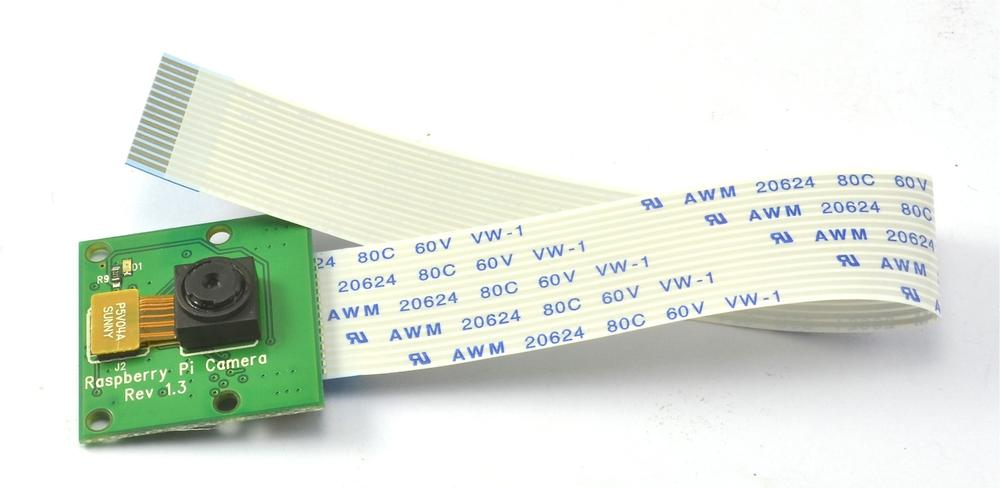
\includegraphics[width=0.4 \textwidth]{pi_cam.png}
	\captionof{figure}{Raspberry Pi Camera Rev. 1.3}
	\label{fig:pi_cam}
\end{figure}
Dette er valgt af flere årsager:
Det er lavet til at køre på en Pi, det er billigt og det opfylder samtlige krav fra kravspecifikationen.
PC'en skal modtage et videofeed fra Kontrolenheden via Wifi. 
Derfor skal Pi'en opsættes til at fungere som en videostreamserver. 
Dette gøres ved at bruge følgende to programmer:
\begin{itemize}
	\item \textit{motion} \cite{motion} - som er et program der håndterer videosignaler fra kameraet
	\item \textit{motionEye} \cite{motioneye} - som giver en webbaseret frontend til motion
\end{itemize}
Opsætningen af de to programmer kan findes i bilag \ref{appendix:Opsaetning_af_robotkamera}.

\subsubsection{Enhedstest af videofeed}
For at teste om streamserveren fungerer optimalt, skal der oprettes forbindelse til serveren og verificeres, at der kan læses video derfra. For dokumentation se bilag \ref{appendix:Bilag_enhedstest_videostream}.

Efter testen kan det konkluderes, at der kan oprettes et live stream fra Pi'ens kamera, som kan ses på PC'en. 